\chapter{Detailed System Design}

In the present chapter, we dissect our system bit by bit and describe each component in detail. We have already described how our data is integrated from different data sources, and also how our ER system works. Here we describe the wiki and the web app that uses all those features.  It is important to note that our sole aim while designing the web application (and the entire system) was to reduce manual work of the verifier - so a lot of brainstorming and design changes went in that direction. Any feature or performance improvement in the verification process makes life easy for the verifier. The system has been designed to be able to crowd-source the verification process like others. \\

Another key point which we have kept in mind always while building the system is to make the data gatherers task hassle-free  - that they should universally be able to communicate with the system. Towards this effect they should also be able to keep track of their data, and also update their old data as well. We have already described how we achieve this using json and rest over a Neo4j back-end we call crawl data-store. We have already described how separation of concerns  further help in achieving this as the crawled-data is well separated in crawl data store. \\

\section{Terminology}

\begin{figure}[H]
\begin{center}  
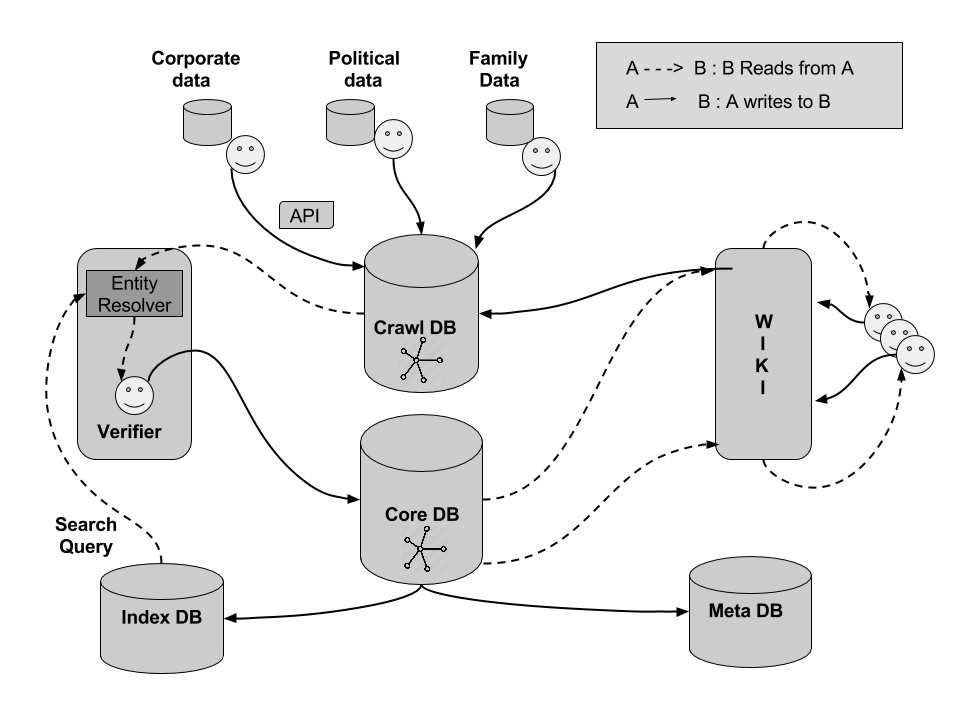
\includegraphics[scale=0.3]{system}
\label{system}
\caption{Detailed Design}
\end{center}
\end{figure}

The detailed design of the system can be see in \ref​{system} We formally define the terminology about the actors and system components here:

\begin{enumerate}
    
    \item Data-Gatherer: An authorized individual or a group of individuals who crawl linked data from different sources. This data can be about entities and relations that belong to any domain supported by our system: political, corporate, sports, bureaucratic, etc. A data-gatherer can use their api-token to push data to our crawl data store using json payload.

    \item Crawl Data Store: The Neo4j data store which stores all non-verified, non-resolved data that data-gatherers push into the system. All data from here is first verified and resolved  

    \item Resolver: A tool that searches over indexed graph data to suggest possible entities for a given entity. ER mechanism has been described in previous chapter in detail. A resolver in essence in our system suggests the probable matches but does not resolve.

    \item Verifier: An authorized person (or a bot) who matches an entity against a possible list of suggestions by the resolver. The only human element on which the system is dependent to be able to push data to the core data store.

    \item Core data store: The Neo4j data store which stores all verified, resolved data that data-gatherers push into the system.  This basically represents our knowledge base - a potpourri of data from different sources.

    \item Registered User: An authorized user who can use wiki to suggest changes to an entity or a relation in the core data store. All these changes are directed to crawl data store.   

    \item Wiki: Part of the web app, where registered users can edit or add information to the core data store.

    \item Meta-DB: MySQL back-end which stores provenance of any info added or changed in the core data store.

    \item Index-DB: MySQL back-end which stores condensed information (and connected information) of all the entities in the core data store. Apache Solr runs on top of it to index this information to help the resolution process. 

    \item Admin: The user with all the privileges in the system - can also delete all indexes, refresh all indexes, see which user/verifier contributed most to the system, change roles of a user.

    \item End user: Non-authorized users that can access information through the web app. They cannot make or suggest any changes to the core data store.

    \item Role: All the authorized users in the system are given a role. The roles are in scoping fashion. The role order from the top is as follows: Admin, Verifier, Crawler, Registered User, End User.  

\end{enumerate}

We have described the tech used in the system in the appendix section. [TODO: did we??]



\section{Data gatherer}

The use case diagram for data gatherer is shown in figure 

\begin{figure}[H]
\begin{center}  
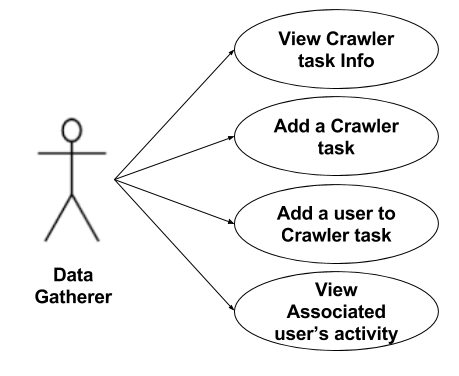
\includegraphics[scale=0.3]{gatherer} 
\caption{Use cases for Data Gatherer}
\label{fig:gatherer}
\end{center}
\end{figure}

use case diagram


  -- they should universally be able to communicate with the system, and should be able to keep track of their data, and also update their data as well, the data should be well seperarted in crawl data store - taskid, userid, tokens -- authentication, api description
  there we talked about json, hwre we talk about api, and metada saved with it
  --va;idations in api in tendem with the data model described  \\
-api snapshot
of what is the view
what is the resulkt from prstman

\section{Resolver and verifier}

verifiers/moderators 
use cas edigarm
-- valid url checked again --
to reolve mean: give a uuid and a relid 

they should be focussed on investigating the links --- show them bext possible results \\

selection algo
and then search -- search query explained in diff section
explain match view, explain diff view
colors in diff view
session checks - resume task
ribust validation chekcing --- no data should get go to worng core data object
locks parallization = apscheduler lib python
views, jaro, search query, view plavcement, diff
jaro useful in some cases only
phonetic serves the purpose, more algos can be fit in
diff new labels, new props, type, conf props, -- name, aliases, lists - mvps!! 
lists and mvps handling imp \\


\subsection{Guideline for the verification task}

a mini-guide to manual verification -- reema sarkar -- [an image]
very imp as only write happens through verifier
shortest path
expand on nodes in neo4j yuvraj singh a falase case can describe
examples of connection --- between sons etc. 
screenshots verifier \\
 

\section{Authorized User and Wiki}
registered users
wiki
use case diagram
explain the design all goes into crawldb
all is verfied- always 
screenshots
read api
wiki \\


\section{Provenance}

provanance
screenshots can be seen by users
how is it done
when verifier verifies
explain
all inputs that we track
see the fn \\

\section{Admin}
admin:
delete index
refresh index
eleveate users
verfier contributions
bots


\section{End user}
end users:
read profiles
see connections
cypher read query - explain - etc.
limit automatically
viz
provenance view
sign up\\

database model er diagrm sanphot meta db - index table also include?? [left] \\